% TEMPLATE for Usenix papers, specifically to meet requirements of
%  USENIX '05
% originally a template for producing IEEE-format articles using LaTeX.
%   written by Matthew Ward, CS Department, Worcester Polytechnic Institute.
% adapted by David Beazley for his excellent SWIG paper in Proceedings,
%   Tcl 96
% turned into a smartass generic template by De Clarke, with thanks to
%   both the above pioneers
% use at your own risk.  Complaints to /dev/null.
% make it two column with no page numbering, default is 10 point

% Munged by Fred Douglis <douglis@research.att.com> 10/97 to separate
% the .sty file from the LaTeX source template, so that people can
% more easily include the .sty file into an existing document.  Also
% changed to more closely follow the style guidelines as represented
% by the Word sample file. 

% Note that since 2010, USENIX does not require endnotes. If you want
% foot of page notes, don't include the endnotes package in the 
% usepackage command, below.

% This version uses the latex2e styles, not the very ancient 2.09 stuff.
\documentclass[letterpaper,twocolumn,10pt]{article}

\newtheorem{theorem}{Theorem}[section]
\newtheorem{lemma}[theorem]{Lemma}
\newtheorem{proposition}[theorem]{Proposition}
\newtheorem{corollary}[theorem]{Corollary}

\newenvironment{proof}[1][Proof]{\begin{trivlist}
\item[\hskip \labelsep {\bfseries #1}]}{\end{trivlist}}
\newenvironment{definition}[1][Definition]{\begin{trivlist}
\item[\hskip \labelsep {\bfseries #1}]}{\end{trivlist}}
\newenvironment{example}[1][Example]{\begin{trivlist}
\item[\hskip \labelsep {\bfseries #1}]}{\end{trivlist}}
\newenvironment{remark}[1][Remark]{\begin{trivlist}
\item[\hskip \labelsep {\bfseries #1}]}{\end{trivlist}}

\newcommand{\qed}{\nobreak \ifvmode \relax \else
      \ifdim\lastskip<1.5em \hskip-\lastskip
      \hskip1.5em plus0em minus0.5em \fi \nobreak
      \vrule height0.75em width0.5em depth0.25em\fi}
      
\usepackage{multirow}

\usepackage{usenix,epsfig,endnotes}
\begin{document}

%don't want date printed
\date{}

%make title bold and 14 pt font (Latex default is non-bold, 16 pt)
\title{\Large \bf Secure Logic Synthesis for Integrated Circuit Obfuscation}

%for single author (just remove % characters)
\author{
{\rm Your N.\ Here}\\
Your Institution
\and
{\rm Second Name}\\
Second Institution
% copy the following lines to add more authors
% \and
% {\rm Name}\\
%Name Institution
} % end author

\maketitle

% Use the following at camera-ready time to suppress page numbers.
% Comment it out when you first submit the paper for review.
\thispagestyle{empty}

\section{Introduction}

The cost of setting up a semiconductor foundry, also referred to 
as a \emph{fab}, 
has been increasing with technology scaling, and is 
currently upwards of \$5 billion~\cite{FoundryCost} for 
cutting-edge fabrication.
As a result, 
many semiconductor design companies have 
adopted the \textit{fabless} model, i.e., they outsource integrated circuit (IC) fabrication to one of a few large commercial IC foundries, often located off-shore. 
As per a recent study~\cite{}, 
four out of the 
top five semiconductor foundries by 
volume are located outside the United States. Most other countries  
either do not have a commercial 
foundry on-shore, and others that do only have access to low-end fabrication technology.  

The fabless model comes with the risk of compromising the 
designer's intellectual property (IP), i.e., the design of chip. 
When a designer outsources a chip for fabrication, the 
foundry obtains full access 
to the chip's layout (effectively a chip blue-print), 
from which it can 
recover its Boolean logic gate-level 
netlist and its 
Boolean 
functionality 
[Citation here? Shall we say IC extraction?]. 
An untrusted 
foundry can sell the designer's IP 
to its competitors or produce and sell extra copies of the 
chip. 
In many cases, the chip might implement proprietary 
protocols or algorithms --- the designer stands to loose competitive 
advantage if these are revealed to competing firms. 
[proprietary security protocol -- if revealed, security compromised?] 
[More citations to indicate that industry/DoD etc care about this?]  

%a heightened risk of intellectual property (IP) theft, 
%laws are lax  or weakly enforced. Hardware IP theft 

%However, this comes at the expense of trust. 
%How can the design company trust that the off-shore (untrusted) foundry has not {pirated its intellectual property} (IP), or maliciously modified the IC by inserting a hardware backdoor, commonly referred to as a {hardware Trojan}, in the chip? 
%Hardware IP theft and Trojan insertion have been recognized as 
%significant threats to the economic viability of outsourced 
%IC fabrication, and to the security of 
%ICs used in 
%areas such as
%critical infrastructure (for instance, communication networks, the smart grid and the emerging internet-of-things), national defense and consumer electronics. 

Logic locking, a technique first introduced by Roy et al.~\cite{}, 
is a promising solution to protect the designer's IP from 
being thieved by an untrusted foundry.\footnote{This technique has 
also been referred to as logic obfuscation~\cite{} and logic encryption~\cite{} in the literature. However, following the lead of Roy et al., we will use the term logic locking throughout.}  
Logic locking works by inserting 
additional gates, referred to as \emph{key gates}, 
in a Boolean 
logic netlist with 
side-inputs that are referred to as \emph{key bits} and 
stored in a key register. 
The netlist functions as intended \emph{only} 
for a certain key, and provides ``junk" 
outputs otherwise. 

The correct key, i.e., 
the key bits that produce the designer's intended 
functionality, 
is known to the designer but not to the foundry. The foundry manufactures the chip and ships the manufactured parts to the 
designer. The designer activates the chips by loading the 
correct key into the key register. 
The security of logic locking 
is premised on the foundry not knowing the correct key.
If the correct key is compromised, the foundry learns of the 
chip's functionality.\footnote{In fact, the protocol proposed by Roy et al. introduces two keys --- a master key that is common to each chip, and a per-instance chip key. See Section~\ref{sec:discussion} for more details? [how to word?]} 

The original logic locking procedure proposed by Roy et al. 
inserts XOR/XNOR gates at randomly chosen locations in the 
net-list. However, several other logic locking mechanisms have been proposed in literature that use different types of key gates or 
different procedures to insert key gates~\cite{}.   
However, recent work by Princeton et al.~\cite{} has 
established 
that \emph{all} of these techniques 
are vulnerable to attack \emph{if} the 
untrusted foundry obtains a 
working copy of the chip, i.e., 
a chip activated with the correct key. 
Note that the foundry cannot directly 
probe the activated chip for the key, but instead 
must infer it from 
the chip's input/output (IO) functionality.   
Princeton 
et al.~\cite{} propose an iterative, SAT-based procedure 
that successfully recovers the correct key for large 
circuits locked 
with a number of techniques proposed in literature. 
[Concurrently, El Massad proposed identical attack for IC camouflaging, that addresses a slightly different defense mechanism.]

Princeton and El-Massad's work has established that 
existing logic 
locking mechanisms are insecure, but 
under \emph{conservative}  
assumptions on the attacker's capabilities.
[Is it clear what we mean? Maybe, under impractical assumptions..] 
That is, for the
attack to succeed, the attacker, i.e., the foundry that is fabricating the chip,must have access to a previously fabricated and 
activated copy of the chip.
Such a strong attack model 
is unrealistic in several scenarios of 
practical interest. 

***Flesh out this para
For one, a foundry may not be able to 
acquire a working copy of a chip that is  
non-consumer electronics [better word/phrase]. 
These include chips designed by government entities [satellites/military 
hardware/critical infrastructure]. Second, even for consumer electronics, first time chip is being taped out [typically when locking is most critical]. 
Finally, locking used to obfuscate an algorithm/mechanisms that has no observable impact on I/O, btu for instance, only on timing/speed. 

So far, the implicit assumption has been that logic locking 
is secure in the more practical setting in which the 
foundry does \emph{not} have access to a working [activated?] chip. 
In this paper, we examine this assumption critically. 
  

 
   





 
 






The rest of the paper is organized as follows. Section 3 

\section{Background: Circuit Locking}

\paragraph{Example} An example of a locking synthesis procedure is the following. Take the behavioral description $f$ and do conventional (locking-free) synthesis to obtain a gate-level implementation. Select $m$ internal wires in the resulting circuit uniformly at random, and associate each with a distinct key bit. Depending on whether the corresponding key bit is 0 or 1, insert either an XOR gate or an XOR gate along each wire, with one input of the gate connecting to the wire's driver and the other input dangling (this is illustrated in Figure ??). Replace each XNOR gate with an XOR gate followed by an inveror then use DeMorgan's laws to move these inverters to random locations up or down the netlist. Provide the resulting netlist as the synthesis output.

\newcommand{\dummyfig}[1]{
  \centering
  \fbox{
    \begin{minipage}[c][0.20\textheight][c]{0.45\textwidth}
      \centering{#1}
    \end{minipage}
  }
}

%% This part makes a figure
\begin{figure}[h]
  \dummyfig{Dummy Figure Label} 
  \caption{A BDD representing the function $f = a \equiv b$. The high and low children of a decision node are discriminated by using a solid (dotted) line to draw the edge leading to the high (low) child.}
  \label{fig:dummy1}
\end{figure}

The reader can see that such an output satisfies the first correctness criterion in Defintion ??. With careful selection of wires in the second step, it is conceivable that it can be made to additionally satisfy the second correctness criterion. However, as we will see later, the procedure does not satisfy our condition for secure synthesis, and as such, must not be considered secure. We use this example locking procedure for its simplicity to illustrate how a basic locking procedure might work. The mechanism was proposed by \cite{} as part of a larger ``purely combinational" IC activation scheme and is known in the lierature as XOR locking \cite{}. It is worth noting that the authors specify that to minimize impact on the delay characteristics of the final chip, all critical paths in the netlist must be avoided when selecting wires for XOR insertion in Step ??.
\section{Secure Synthesis}
In this section, we argue that XOR locking (Section ??), and to the best of our knowledge, must not be considered secure; as they all fail to satisfy basic requirement of any information hiding scheme with no c. We Following the principles of secure design, we do not assume a synthesis procedure to be secret; rather we base our security on the secrecy of the correct key $k^*$.

\subsection{A Necessary Condition}
Intuitively, a synthesis procedure must at a minimum make it ``hard" --- if at all possible --- for a malicious entity at a fab to recover the correct key from an encrypted design. To make an analogy to the traditional setting of encryption, this is similar to say that it must be hard or impossible for an eavesdropper to correctly guess a sender's secret key simply by observing encrypted communication between the sender and a receiver \footnote{the settings are not exactly the same as unlike most settings where encryption is used, here the ``eavesdropper" only gets to read a \emph{single} message; the sender also gets to change the encryption key prior to sending a new communication}. Cryptographic protocols usually ensure this by making key deduction equivalent (or at least as hard as) solving a computational problem known to be xxxx hard. Common examples are integer factoring and the discrete logarithm problems \cite{}. This is know as the computational hardness approach to security \cite{}.

Another approach, the information theoretic one \cite{} is to xxxx make a plaintext absolutely independent of the ciphertext, \footnote{In cryptography, this is known to be possible to achieve only when the key space is as large as the message space \cite{}. Therfore, information theoretic security, while intuitively preferrable, is usually foregone in xxxx of computational security, which is possible to achieve even given key spaces of limited size (security is parameterized by the key length)}where independence is xxxx in a probabilitstic sense, i.e., if $X$ is a random variable that denotes the plaintext, and $Y$ is the random variable that denotes the ciphertext, then the probability distributions of the two variables must satisfy:

$$ P(X|Y) = P(X) $$

In our setting, we seek to protect the locking key; and what the attacker has access to is an encrypted netlist output by a synthesis procedure as defined in Section ??. We there argue that a \emph{necessary} condition of secure synthesis is:

\begin{proposition}
A locking synthesis procedure as defined in Section ?? is secure only if for every behavioural description $f$, the synthesis output $C$ and key $K$ satisfy 
$$ P(K|C)=P(K) $$
where the probabilities above are computed assuming each of the $2^{2^n}$ behaviours that can be provided as input to the synthesis procedure --- are equally likely, and that for each behaviour, all descriptions are equally likely to be provided as input.
\end{proposition}

The condition in Proposition ?? ensures that given the unencrypted netlist, knowledge of the encrypted netlist does not reduce uncertainty about the locking key. %Is this condition sufficient by itself to guarantee impossibility of key recovery? No. As a counter-example, consider a synthesis procedure that produces, for an input behavioral description, a implementation that, for all keys other than the correct one, behaves as specified by the input description, for all inputs save one (a fixed value for all keys). The construction in Figure?? is one example of such implementation The comparator checks wether the input key . Such synthesis procedure is clearly secure according to Condition 1; the input correct key value is not used at all when constructing the encrypted design; therefore the locked design produced is the same for all input keys, i.e., it is independent of the correct key value. Such a locking 
%We therefore introduce another condition for secure synthesis:
%\begin{proposition}
%A synthesis procedure as defined in Section ?? is secure only if 
%\end{proposition}
%Such a condition rules out procedures like the one in Figure ??.
Note that we assume that for every behaviour, all descriptions are equally likely \footnote{It can be argued that not all descriptions are likely for a given desired behaviour; e.g, if the circuit is required to produce $0$ identically as output, this is more likely to be specified in VHDL as an output port being set to zero; rather than the AND of two intermediate signals that are complements of each other. This is just an extreme example; a reader experienced in VLSI design will identify more realistic ones.}. This is why the condition is necessary.

\subsection{Are Existing Schemes Secure?}
In Section ??, we report experimental evidence that a sample locking procedure --- XOR locking --- is not secure as a simple attack manages to recover more bits of the correct key that should be possible by random chance. Here, we make make an informal argument why --- due to the way they work in general --- none of the existing locking schemes satisfies our necessary condition for secure synthesis.

A quick look at locking schemes that have been proposed in the literature reveals a general trend to refrain from perform locking on the RTL; but to rather do it on some a technology-mapped netlist (as in the case ofo \cite{} and \cite{}), or unspecified (but implied to be a network, as in \cite{}). This to justifiable to some extent: one can argue that locking is more easily done on a network-representation of a circuit; rather than an abstract form of desired behaviour (such as a Verilog or VHDL code). To see this, consider that the opportunities for modification are generally higher in a Boolean network than in a corresponding RTL description (a single Verilog line of code such as z = a + b where a and b are 32-bit registers will be converted by a Verilog compiler to a network with at least 32 XOR gates, each of which is candidate for modification by a locking algorithm, e.g. one that inserts XOR gate). The second correctness criterion is also easier to satisfy when working on Boolean network rather than RTL. For example in the context of XOR locking, one can use an automatic test pattern generation tool to make sure that two stuck-at-faults at the selected wires do not cancel each other out, thereby rendering some incorrect key equivalent to the correct one, in the sense that applying the incorrect key results in correct circuit behaviour. Given that ATPG tools accept netlists as input, it is attractive to defer locking till at least some form of synthesis has been performed (e.g, until a corresponding multi-level network has been constructed by the synthesis tool, as a first step to prepare the network for optimization).

In this paper, we argue that performing locking post-synthesis (or in general, after some optimizing transformation has been applied on the RTL) in a logic locking scheme, introduces a subtle vulnerability in the scheme. The vulnerability comes about as a result of the fact that --- Unlike ``raw" RTL (pre-synthesis) --- in an optimized network, different parts of the network are no longer ``independent" of each other as they were before synthesis. Consider, for instance, an optimizing transformation that looks for sequences of inverters in a netlist, and replaces each with a single (or no) inverter (preserving the Boolean function implemented by the network). This is a very simple transformation to apply on a circuit netlist, and one that presumably any worthwhile logic synthesis tool should implicitly or explicitly perform. Now assume that the step of moving inverters up and down the netlist in the XOR locking scheme is removed from the procedure. A sequence of two inverters will then be a dead giveaway that the correct value of the key bit feeding the preceding XOR gate is a 1 (and so an inverter has been placed by the locking procedure after the XOR gate to ensure the first correctness criterion is satisfied). This is of course a trivial example, and it only fair to assume that the authors of the XOR locking procedure introduced the inverter moving step to prevent such an easy attack. Our point is that unless the procedure guarantees \emph{by construction}, and \emph{for every circuit}, that each key is equally likely regardless of the procedure's output (as ensured by our necessary condition for secure synthesis), such a locking procedure should \emph{not} be considered secure.

We now propose a candidate locking procedure that not only meets our necessary condition for secure synthesis, but also allows to easily ensure the correctness criteria of locking synthesis are satisfied. We first provide a brief introduction to a concept in  that is critical to understanding our technique, that is of binary decision diagrams. 
%A reader familiar with binary decision diagrams can skip directly to Section ??.

\subsection{Binary Decision Diagrams}
A binary decision diagram (BDD) is a way of representing a Boolean function in terms of a graph that describes the Boolean calculations performed by the function. Given an assignment to the input variables of the function, an evaluator starts at the root of the diagram and proceeds by selecting one of the two children the current node, based on the value of the variable associated with the node. This continues until the evaluator reaches a leaf node, which specifies the value taken by the function at that particular sequence of input values. As an example, a BDD for representing the function $f = a \equiv b$ is shown in Figure ??.

%% This part makes a figure
\begin{figure}[h]
  \dummyfig{Dummy Figure Label} 
  \caption{A BDD representing the function $f = a \equiv b$. The high and low children of a decision node are discriminated by using a solid (dotted) line to draw the edge leading to the high (low) child.}
  \label{fig:dummy}
\end{figure}

More formally, a BDD can be defined as a rooted directed acyclic graph with two types of nodes: \emph{decision} and \emph{terminal} nodes. A terminal node can be either a $0$-terminal or a $1$-terminal, and there can be at most two terminal nodes in a BDD. Each decision node, $N$, is labeled with a variable $V_N$ and has two child nodes: a low child and a high child. The edge from $V_N$ to its low (or high) child represents an assignment of $V_N$ to $0$ (respectively $1$). A path from the root node to the $1$-terminal represents a variable assignment for which the Boolean function is true. Similarly, a path to the $0$-terminal represents a variable assignment for which the Boolean function is false. Note that given a BDD representation of a function, we can easily build a Boolean circuit that decides the function, for instance, by replacing each decision node $N$ with a 2-to-1 multiplexer that uses $V_N$ the its select line. This is illustrated in Figure ???.

\begin{figure}[h]
  \dummyfig{Dummy Figure Label} 
  \caption{A BDD representing the function $f = a \equiv b$. The high and low children of a decision node are discriminated by using a solid (dotted) line to draw the edge leading to the high (low) child.}
  \label{fig:dummy}
\end{figure}

BDDs as a way of representing Boolean functions are special, in that a BDD is a canonical representation of its corresponding Boolean function:, i.e., if we fix the input variable order, there is only one way to represent a Boolean function using a BDD \cite{}. Moreover, unlike a truth table (another canonical representation), the size of a BDD is not always exponential in the number of input variables. These two facts together form the basis for the data structure use in a wide variety of applications \cite{}. Canonicality, in particular, plays a key role for our construction of a secure synthesis procedure, as will become apparent shortly.
%\footnote{One might wonder why we require the to be probably only; rather than requiring the outputs for both description-key pairs to be identically distributed. We argue that since an encryption key here is used only one time}

%An overview of the various logic locking technique that has been proposed in the literature:
\subsection{A Secure Synthesis Procedure}

We now describe a locking synthesis procedure that meets the necessary condition for security introduced in Section ??. A striking feature of our procedure (or perhaps the necessary condition) is that it enables any transformation to be applied on resulting implementations (provided of course the transformation is functionality-preserving), without compromising security at all. We formalize this in the following lemma.

\begin{lemma}\label{simple}
Let $T$ be a functionality-preserving transformation, and denote by $s \circ t$ the (correct) synthesis locking procedure we obtain by composing $T$ with a locking synthesis procedure $s$. If $s$ satisfies the necessary condition for security of Proposition ??, the so does $s \circ t$. 
\end{lemma}
The proof of the lemma is straightforward.

Our synthesis procedure takes the RTL description provided as input, and uses it to constructs a corresponding Boolean network. The BDD representation of the output variable's Boolean function is then computed (recall that we are assuming an RTL description of a single-output circuit). This BDD is then written in a compact form (), and modified to obtain a ``locked BDD". The locked BDD is then converted to a Boolean circuit, which is finally provided as output of the synthesis procedure. If a designer so wishes, they can then feed this circuit to a logic synthesis tool to further optimize it (or to perform technology mapping and obtain an implementation in terms of logic gates); thanks to Lemma \ref{simple}, they can be sure that these further operations on the circuit will in no way affect the security property.  We next describe each of the xxxx steps in detail, then prove that our procedure satisfies the necessary condition for secure synthesis in Section ??.

%The first step
In a standard BDD representation, every node can be thought of as representing an ``intermediate" Boolean function that defines the behavior of the ``overall" Boolean function for a specific partial variable assignment (the assignment represented by the path from the root to the node in question). Let $N_h$ and $N_l$ be the high and low children, respectively, of decision node $N$, and let $f_{I}$ be the Boolean function represented by node $I$.  We can then write,

\[f_N=V_N f_{N_h}+V_N' f_{N_l}\]

Note that if we switch the polarities of $N_h$ and $N_l$, the function represented by node $N$ becomes:

\[f_N^*=V_N' f_{N_h}+V_N f_{N_l}\]

We convert the standard BDD representation to a ``compact" representation in which a decision node $N$ represents both functions, and we signify this in a graph using ``bubbled" nodes. An incoming edge to a decision node $N$ can either terminate at the ``main" part or the ``bubble" part of $N$, to indicate which of the two functions $f_N$ and $f_N^*$ defines the behavior of the overall function for the corresponding partial variable assignment. An BDD can be converted into this form by simply looking for ``complement" nodes (a pair of nodes labeled with the same variable and that has the same children as each other; with different polarities), and replacing each pair with a single ``bubbled" node, preserving original ROBDD edge connectivity. Note that looking for such nodes is easy (we need to perform $O(N^2)$ comparisons, where $N$ the maximum number of nodes at any level in the BDD). An example is shown in Figure ??. Note that since the conversion procedure operates on BDDs --- a canonical representation --- and is deterministic, the resulting representation of the Boolean function must also be canonical. We call the new compact representation a \emph{bubbled} BDD.

\begin{lemma}

\end{lemma}

\begin{figure}[h]
  \dummyfig{Dummy Figure Label} 
  \caption{A BDD representing the function $f = a \equiv b$. The high and low children of a decision node are discriminated by using a solid (dotted) line to draw the edge leading to the high (low) child.}
  \label{fig:dummy}
\end{figure}

\paragraph{Encryption Procedure}  To encrypt the new BDD, we pick $k$ nodes at random and insert a new node for each as a descendant, in the manner shown in Figure ??. Each of the new $k$ nodes is then labeled with the variable corresponding to a distinct key bit. If the value of the corresponding key bit is $1$, the polarity of node $N$'s children with respect to the new key node, is preserved; otherwise, children polarities are flipped (low becomes high and high becomes low). %The resulting BDD is then fed into a synthesis tool (after conversion into a circuit) to obtain the final implementation.

\begin{figure}[h]
  \dummyfig{Dummy Figure Label} 
  \caption{A BDD representing the function $f = a \equiv b$. The high and low children of a decision node are discriminated by using a solid (dotted) line to draw the edge leading to the high (low) child.}
  \label{fig:dummy}
\end{figure}

%\begin{figure*}[!htb]
%\centering
%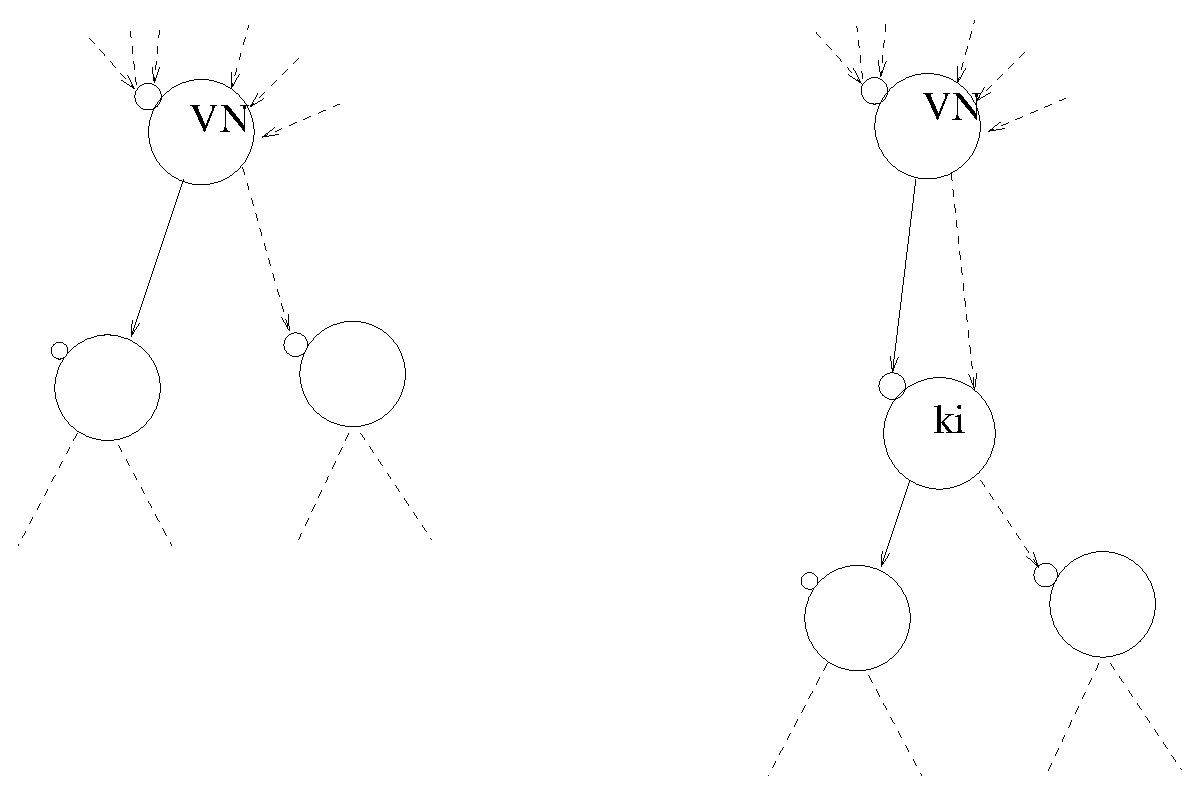
\includegraphics[scale=.5]{bubble_encrypt.eps}
%\caption{Digraph.}
%\label{fig:digraph}
%\end{figure*}

\begin{lemma}
Let $G_{k'}$ be the graph we get by eliminating key nodes in an encrypted BDD and making connections in accordance with the value of $k'$, and then replacing each bubbled node with its ``regular'' equivalent. Then $G$ is a BDD.
\end{lemma}

\begin{proof}
Assume not. Then $G$ must either contain nodes whose children are isomorphic (impossible, since there could not have been any in the original graph), or $G$ must contain subgraphs that are isomorphic. A pair of such subgraphs cannot be rooted by complement nodes, by definition; they also cannot be rooted by a pair of nodes ``originating" from different bubbled nodes (it would mean the original graph also had isomorphic subgraphs). No other possibilities remain, and thus no such pair of subgraphs can exist in the $G$. Hence, $G$ is also an ROBDD.
\end{proof}

\begin{lemma}
Each $G_{k'}$ is a distinct BDD.
\end{lemma}

\begin{theorem}
$s^{*}$ satisfies the necessary condition for secure synthesis of Proposition ??.
\end{theorem}

\begin{proof}
Let $f$ be the input description to $s*$, and denote by $c_k$ the output we get . Note that $c_k$ is a random variable. We need to show that for each $k\in K$, there exists a description $f_k$ that, when locked with $s^{*}$ using $k$ as a key, we get $c_k$; with the same probability for all $k$. This description is simply the Boolean circuit corresponding to $G_{k}$ for each $k$. Due to the fact that BDDs are canonical, we know we will obtain $G_{k}$ at the end of Step 1 of the procedure, if we provide such circuit as input to the locking procedure with $k$ as the locking key. All we need now is to show that the subset of nodes selected in the locking step is as likely to have been selected by $s^{*}$ as the corresponding set of nodes in the BDD of $f$, but since $s^{*}$ selects decision nodes for locking uniformly at random, this direcctly follows.
\end{proof}

this esse consists of inserting XOR gates at random plac
%In a bubbled BDD, rather than 
%Encryption in a bubbled BDD corresponds to inserting new bubbled nodes 


\section{Experimental Evaluation and Results}



\begin{table*}[ht]
\centering
\caption{Performance of hill-climbing MSE attack on 11 sequential benchmarks from the MCNC set. Numbers are average number of key bits correctly recovered by attack for 5 runs on each benchmark.}
\label{my-label}
\begin{tabular}{|l|l|l|l|l|l|l|l|l|l|l|l|l|}
\hline
\multirow{4}{*}{} & \multicolumn{12}{c|}{Number of Key Bits}                                                                                                                        \\ \cline{2-13} 
                  & \multicolumn{4}{c|}{32}                             & \multicolumn{4}{c|}{64}                             & \multicolumn{4}{c|}{128}                            \\ \cline{2-13} 
                  & \multicolumn{3}{l|}{Correctly Recovered} &          & \multicolumn{3}{l|}{Correctly Recovered} &          & \multicolumn{3}{l|}{Correctly Recovered} &          \\ \cline{2-13} 
                  & Min         & Max         & Avg.         & Time (s) & Min         & Max         & Avg          & Time (s) & Min         & Max         & Avg          & Time (s) \\ \hline
dk16              &           &           & 24.5         &          &           &           &         44 &          &           &           &          &          \\ \hline
ex1              &           &           & 23.7         &          &           &           &            &          &           &           &          &          \\ \hline
keyb             &           &           & 22.4         &          &           &           &          &          & 
&           &          &          \\ \hline
planet1             &           &           & 21.13         &          &           &           &          &         &           &           &          &          \\ \hline
planet             &           &           & 20.8         &          &           &           &      33    &         &           &           &          &          \\ \hline
s1a             &           &           & 20         &          &           &           &          &      &           &           &          &          \\ \hline
s1             &           &           & 18          &          &           &           &         37 &         &           &           &          &          \\ \hline
sand             &           &           & 17.8         &          &           &           &        36.6  &         &           &           &          &          \\ \hline
scf             &           &           & 21.2         &          &           &           &         40.2 &         &           &           &         75 &          \\ \hline
styr             &           &           & 18.8         &          &           &           &         38.6 &         &           &           &          &          \\ \hline
tbk             &           &           & 22.2         &          &           &           &         36 &         &          &           &          &          \\ \hline

\end{tabular}
\end{table*}

%Results below are for the case where XOR gates are inserted at random, and inverters are left where they are (no moving inverters up and down the netlist). No care is taken to avoid critical paths in the netlist when inserting inverters, but output wires are avoided. 

%When initial guess is selected at random, 15-19 bits of a 24-bit key are successfully recovered. (didn't study the effect of key gate locations on performance of the attack)

%24, 21, 22, 23, 22  32
%7, 15, 11, 14, 13  48
%17, 16 64

%Even when the initial guess is the exact complement of the correct key, a significant portion of key bits is correctly recovered.

\subsection{Performance Evaluation on Benchmark Circuits}
To provide an insight on the once can expect from locking a VLSI design using our procedure, we implement our procedure using PHP and the ABC system \cite{} for BDD construction, and use the implemented tool chain to encrypt sequential circuits from the MCNC benchmark suite. As a baseline, we also report the overhead of locking the same circuits using XOR locking. The results are reported in Table ??.

We note that one can use other, more BDD-targeted synthesis tools (the BDS and FDD tools from the Universities of Amherst and Toronto, respectively for example) in place of ABC as a backend --- to obtain implementations with potentially less area and delay overheads. Whether such tools are better equipped to synthesis circuits resulting from our locking synthesis tool-chain, we leave as topic for future work.

\begin{table*}
\caption{Area and delay overheads of our BDD-based obfuscation technique when implemented on the alu4 benchmark. }
\begin{tabular}{ | c | c | c | c | c | }
\hline
 Benchmark Name & Area Overhead (32-bit) & Delay Overhead (32-bit)  & Area Overhead (64-bit) & Delay Overhead (64-bit) \\
\hline
bbara.kiss2&3.91&1.36&5.72&1.68\\
bbsse.kiss2&2.22&1.27&3.16&1.42\\
beecount.kiss2&4.04&1.88&11.60&2.36\\
cse.kiss2&1.72&1.09&0.00&0.00\\
dk14.kiss2&2.55&1.50&4.08&1.60\\
dk15.kiss2&3.56&1.32&5.88&1.70\\
dk16.kiss2&1.46&1.16&1.94&1.24\\
dk17.kiss2&3.49&1.60&5.69&1.69\\
dk512.kiss2&3.37&1.45&5.35&1.58\\
donfile.kiss2&1.75&1.36&2.66&1.38\\
ex1.kiss2&1.68&1.13&2.28&1.20\\
ex2.kiss2&2.13&1.38&3.08&1.53\\
ex3.kiss2&3.23&1.53&5.32&1.58\\
ex4.kiss2&2.76&1.48&4.31&1.69\\
ex5.kiss2&3.11&1.41&5.18&1.63\\
ex6.kiss2&2.96&1.30&4.29&1.42\\
ex7.kiss2&3.34&1.47&5.40&1.60\\
keyb.kiss2&1.70&1.08&2.27&1.15\\
kirkman.kiss2&2.17&1.17&3.02&1.23\\
mark1.kiss2&2.66&1.55&3.68&1.84\\
opus.kiss2&2.61&1.41&4.06&1.52\\
planet1.kiss2&1.26&1.04&1.61&1.22\\
planet.kiss2&1.27&1.27&1.61&1.26\\
s1a.kiss2&1.45&1.15&1.87&1.22\\
s1.kiss2&1.33&1.10&1.66&1.18\\
sand.kiss2&1.31&1.13&1.56&1.22\\
scf.kiss2&1.14&1.06&1.33&1.04\\
sse.kiss2&2.29&1.24&3.20&1.47\\
styr.kiss2&1.36&1.03&1.72&1.09\\
tbk.kiss2&1.34&1.00&1.47&1.10\\
train11.kiss2&3.95&1.72&&\\
\hline
\end{tabular}
\end{table*}

%c880 (no random restarts) 
%24 17 72.38 18 66.75 14 43.2 20 67.23 16 82.57

%32 20 89.55 23 56.06 20 115.88 22 125.43 21 140.16

%48 36 223.74 37 209 31 164.34 38 151.75 30 128.42

%64 43 258.8 45 413.56 45 371.98 43 224.99

%80 48 518.51 57 488.26 62 591.109 55 556.18

%96 70 539.96 69 636.91 73 819.2 73 660.38 72 795.82

%112 74 968.78 89 1079.58 74 698.56 89 1090.43 72 1086.43

%128 94 1403.94 92 1234.59 82 1166.71 94 1285.91 94 1243.16

%c880 - 32-bit with random restarts
%Number of correctly recovered bits      Time Taken (s)
%23                                                         1645.87
%24                                                         1458.24
%27                                                         1667.95
%25                                                         1653.95
%25                                                         1813.47

%I ran the attack on c1908 (a bigger benchmark) encrypted with a 24-bit long key.. For five random initial key guesses: from 12 to 15 bits of the key were correctly recovered.

%For 64-bit keys:
%Number of correctly recovered bits      Time Taken (s)
%48                                                         5385.41
%44                                                         4790.02
%48                                                         4686.72
%48                                                         5035.48
%47                                                         3780.07

%For 128-bit keys:
%Number of correctly recovered bits      Time Taken (s)
%101                                                       8585.73
%96                                                         8311.26
%93                                                         8164.93
%94                                                         8341.93
%92                                                         6334.29

%BDS actually just finished synthesizing the new smaller BDD, but the results are similar to those of ABC.. The area overhead is about 19X and the delay overhead is still 2.4X




%Number of gates: 632
%Area: 1088080.00
%Delay: 6.63

%For BDS global BDD synthesis (when fed with BDD rep. generated by ABC):

%Number of gates: 620
%Area: 1060240.00
%Delay: 7.50

%When encrypting with 16 key gates: 
%Number of gates: 1048 
%Area: 1765984.00
%Delay: 12.19

%When encrypting with 32 key gates:
%Number of gates: 1360
%Area: 2330672.00
%Delay: 9.51

%1508928.00 instead of 1765984.00 (1.4X instead 1.6X) sound like a more reasonable area overhead for encrypting alu4 with 16 key gates?
%Delay is 13.56


\section{Discussion}
Why randomness

Weakness - key size limited by number of nodes

close to being sufficient - not all descriptions need to be likely

not necessary for procedures with computational guarantees. not clear how to construct such a procedure.
\section{Related Work}
While attractive, XOR-based locking has been shown to suffer from certain weeknesses. Rajendran et al. show that selection of random wires to replace with XOR gates is ineffective to defend against a certain kind of attack. The attack they describe uses a functional chip, and automatic test pattern generation to resolve the correct values of key bits. They also show that unless wires are selected judiciously, an incorrect key applied to the ``encrypted" circuit may not always result in significantly different behaviour. They describe algorithms for wire selection that, they argue, defends against their attack, and maximize 

Since its introduction, logic encryption has been subject to various kinds of attacks. The first known attack, described by JV et. al, leverages VLSI testing principles to decipher the functionality of the camouflaged gate . The attack described by us in the context of camouflaging could also be potentially adapted to work againt logic encryption. Igor also proposes an attack that uses test patterns provided by the designer to guide a hill climbing search for the correct key.

A common thread across all published attacks is that they generally require some level of access to input-output behaviour information of the circuit. JV's attack assumes access to a functional IC, which the fab presumably acquired from the market after fabricating the first batch. The same things holds for our attack. Igor's attack assumes access to test patterns provided by the designer.


\section{Conclusion}

{\footnotesize \bibliographystyle{acm}
\bibliography{../common/bibliography}}


%\theendnotes

\end{document}
